\title{Synthesizing Static Analyses from Examples}
\author{
        Martin Kellogg \\
        University of Washington
            \and
        Everett Maus\\
        Microsoft Corporation
}


\documentclass[10pt,conference]{IEEEtran}

\usepackage{graphicx}
\usepackage{myref}
\usepackage{booktabs}
\usepackage{url}
\usepackage{listings}
\usepackage{color}
\usepackage{tikz}

\begin{document}

\maketitle

\lstset{language=C}

\begin{abstract}

Constructing static analyses requires a great deal of
manual, expert programmer effort. Because of the large amount of
effort required to build a precise static analysis, custom analyses
are rarely deployed by developers, despite their potential
for finding bugs and verifying correctness. Compounding the problem,
the expert researchers who do design novel static analyses often
do not engineer their analyses to the level of practicality that
developers require. We propose a technique
for automatically synthesizing the implementation of analyses
from examples of the desired analysis in action,
reducing the effort required to design, build, and deploy static analysis
tools.

\end{abstract}

\section{Motivation}

A well-designed static analysis (or, equivalently, a type system or
abstract interpretation) can allow developers to find bugs in their
code quickly and with little manual effort, or even avoid entire
classes of errors by verifying that their code can never enter an
undesirable state. However, these benefits come at a cost---developing
such a static analyses requires an expert to spend a long time both
designing and implementing the static analysis (for instance, a static
analysis that checks the types of the arguments to a format string was
novel enough to be published at a recent top-tier software engineering
venue~\cite{format-string-checker}).  Worse, the cost to build such
static analyses means that many that are designed by the research
community are never engineered to the level of practicality and
precision that would be required to run on real-world code, so most
programmers never gain their benefits.

We propose to deploy state-of-the-art techniques from the domain of program
synthesis to allow programmers to specify a static analysis by providing
examples of the code that the analysis should and should not permit.
Our technique then synthesizes an abstract interpretation of the analysis,
which is then mechanically translated to an analysis framework like
the Checker Framework~\cite{checker-framework} or LLVM~\cite{lattner04:_llvm}.
A simple analysis could be specified
with just a few test cases (consider, for example, a function that needs to
be called with arguments that are related more precisely than a typical
type system would allow the programmer to express, like a pair of integers that
must sum to zero---with a few test cases and our technique, an analysis that
enforces this property could be run on an entire industrial codebase).
This will relieve the burden of actually building the infrastructure
required to deploy complex static analyses, so that specialized analyses
with the precision required of industrial-strength tools can be built without
requiring an intimate knowledge of the theory of abstract interpretation,
which will allow non-specialists (like industrial programmers) to easily
build new, customizable static analyses.

We envision a scenario like this: a developer or a researcher comes up with
a new static analysis. To test out their analysis today, they would need
to build the entire static analysis in an existing framework (like the Checker
Framework~\cite{checker-framework}). This requires them to: determine
the lattice and transfer functions used by their analysis (see \secref{ai}),
understand how
to use the framework they choose for implementation, write the implemention,
and finally to test and debug the implementation. Our proposed technique
shortcuts this process: it requires them only to determine the lattice
and then to write a series of examples of the analysis in action, which
should be equivalent to the test suite they would have to write anyway.
Then, they can apply the analysis to the code they care about, and any
place where it fails in practice (with either a false negative or a false
positive) can be added to the test suite from which the analysis
is generated. In this way, our approach allows analyses to be constructed
relatively cheaply and iterated on until they achieve the desired precision.

The technique we describe above requires several pieces:
\begin{enumerate}
\item A parser for annotated programs in the target language.
\item A tool that traverses the abstract syntax tree produced by 1) and
generates constraints on the transfer functions.
\item A tool that takes a lattice and a target language and produces
a set of \emph{sketches} (see \secref{synth}) of the transfer function.
\item A solver that takes the output of 2) and 3) and produces
a complete transfer function.
\item A framework for building static analyses that run on the target language.
\item A tool that translates the output of 4) into a static analysis built in
5).
\end{enumerate}

Off-the-shelf tools can be used for items 1), 4), and 5) above: many
languages support annotations~\cite{jsr308},
modern SMT solvers are fast on most queries~\cite{z3},
and frameworks for building static analyses exist in many common languages
(like the Checker Framework~\cite{checker-framework} for Java). Our tool
must provide 2), 3), and 6). We believe the most difficult parts to
get right (and therefore the most interesting research contribution)
will be in 2) and 3): designing the constraint generation tool and the
sketches so that they capture the static analysis the programmer intended
with a small number of test cases, we believe, is the most challenging
problem. Our proposal for this class therefore focuses on those parts,
leaving 6) as future work.

\section{Background}

\subsection{Abstract Interpretation}
\label{sec-ai}

\begin{figure}
 \includegraphics[width=\linewidth]{parity.png}
 \caption{A lattice of abstract domains and a transfer function
   for plus, for an abstract analysis that tracks the parity of
 a value.}
\label{fig-parity}
\end{figure} 

A static analysis can be formally modelled
as a lattice of \textit{abstract domains} and a set of \textit{transfer functions}
that transform abstract domains to other abstract domains when some
program operator is encountered~\cite{cousot77}. The analysis then proceeds by symbolically
interpreting the program being analyzed, replacing each concrete value with
an abstract domain determined by applying the transfer functions. An example
lattice and transfer function for the plus operator are given in Figure~1.
The analysis shown in Figure~1 is a parity analysis---it keeps track of
whether integers are even or odd. There are also two other possiblities:
the integer could be either even or odd (the ``top'' type) or it could
be \textit{both} even and odd---such as in dead code (represented by the
``bottom'' type). The lattice shows how these abstract domains are related,
with a subset relationship represented by the lines---any abstract domain
with a line going to another abstract domain higher in the lattice is a strict
subset of the higher abstract domain (so, for instance, top contains both
all even integers and all odd integers, so both even and odd are below it in the lattice).
The transfer function shows how the result of the plus operation is related
to its operands. We represent this as a matrix, with the top row and leftmost
column representing the abstract domains of the operands, and the interior
parts of the matrix representing the abstract domain of the result. So,
as an example, if $a$ is odd and $b$ is bottom, then $a + b$ is bottom,
because the entry for odd and bottom in the matrix is bottom.

\subsection{Synthesis}
\label{sec-synth}

The field of program synthesis uses SMT solvers to
automatically build programs based on a set of constraints provided
by the programmer. Modern SMT solvers, such as z3~\cite{z3}, are able
to solve equations involving millions of variables extremely quickly, despite 
the problem they solve (boolean satisfiabilty) being known to be NP-complete~\cite{cook71complexity}. 
These modern solvers allow the synthesis of, for example, memory models for modern architectures
in a few seconds from the architecture's litmus tests~\cite{bornholt17}.
Synthesis works by reducing the constraints provided by the user
(litmus tests, a formal specification, etc.) to a boolean satisfiability
problem, calling the solver, and then translating the result back into
a program. Because the search space for programs is so large, practical
synthesis techniques use \textit{sketches} of the solution to reduce
the search space. A sketch is an outline of the form of the answer,
such as a program with some expressions missing.

\section{Technical Approach}
\label{sec-tech}

This section focuses on the part of the proposed tool that generates
constraints from examples and passes them to an SMT solver. These are
the pieces of the proposed solution that we implemented for this course
project.

\subsection{Lattice and Examples}
\label{sec-input}

The programmer provides three things: a lattice,
an abstraction function, and a set of example programs.

The lattice for the abstract analysis must be provided.
The lattice includes both the abstract domains and a least
upper bound relationship between them. Our tool currently
requires these to be specified in source code, but future
work would include a simple parser that reads this information
from a configuration file. The abstraction function is provided
in a similar manner, and would be similarly provided in a configuration
file in future work. It relates constants to lattice elements.
For instance, the abstraction function for the parity analysis
in \secref{ai} relates all even integers to the \lstinline{@Even}
lattice element.

The examples are code snippets annotated with the
abstract domains (in the same way typed languages have type annotations).
Consider the example below, which is a sample example that a
programmer might write while building a parity analysis like the one
used as an example in \secref{ai}:

\begin{lstlisting}
@Even x = 2;
@Even y = 4;
@Even z = x + y;
\end{lstlisting}

\subsection{The Sketch}
\label{sec-sketch}

Our tool provides a sketch of the transfer function. Most of the
sketch is dedicated to declaring the transfer functions for various
operators. For instance, the code below is the \lstinline{smt2}~\cite{smt2}
code that our tool generates for the plus operator when preparing
a sketch for the parity analysis in \secref{ai} (\lstinline{Elt} is
a special type that can only be inhabited by a lattice element):

\lstset{language=[]Lisp}
\lstset{morekeywords={assert-soft, declare-fun}}
\begin{lstlisting}[columns=fullflexible]
(declare-fun abstract-plus (Elt Elt) Elt)
(assert-soft (= (abstract-plus @Both @Both) @Both))
(assert-soft (= (abstract-plus @Both @Bottom) @Bottom))
...
\end{lstlisting}
\lstset{language=C}

The first line declares the function \lstinline{abstract-plus}, which
is the transfer function for plus. The second and third lines are
\textit{soft constraints}~\cite{bjorner2015nuz},
each of which biases the solver towards returning the top lattice
element for any transfer not involving the bottom element, and the
bottom element for transfers that do involve the bottom element.
There is a soft constraint for each pair of lattice elements; our
example omits all but two.  These constraints are not required to be
satisfied, but the solver prefers solutions in which they are
satisfied to solutions in which they are not.  Though adding soft
constraints does convert the problem from a standard satisfiablity
problem to an optimization problem, because the number of these
constraints introduced is proportional to the size of the sketch, the
impact of these constraints on performance is not problematic---no
matter how large the input, the number of soft constraints generated
is constant.  As a result of the soft constraints, the produced
transfer function will always be sound in underspecified cases; they
have the effect of introducing a default behavior that corresponds
with typical analyses.

Our sketches also include constraints about the mathematical properties
of certain functions. For instance, addition and multiplication must
be commutative.

\subsection{Generating Constraints}
\label{sec-cgen}

To generate contraints from the code sample in \secref{input},
our tool
performs a straightforward dataflow analysis. The analysis
maintains an abstract store and propagates the annotations
through the program using standard dataflow rules (so, for
instance, \lstinline{x} in the example above still has
a \lstinline{@Even} annotation on the third line).
As it analyzes the code, the tool generates
constraints when it encounters a statement that
can be used to constrain a transfer function, like
the third line above (which constrains the transfer function
for plus). The tool generates
the following \lstinline{smt2}~\cite{smt2} constraint:

\lstset{language=[]Lisp}
\begin{lstlisting}[columns=fullflexible]
(assert (= (abstract-plus @Even @Even) @Even))
\end{lstlisting}
\lstset{language=C}

This constraint corresponds to the final statement in the
simple imperative program above.
It is a \textit{hard constraint}---that is, it must be satisfied
by the solver.
\lstinline{abstract-plus} is defined in the sketch (\secref{sketch}) and defines
the transfer function for the plus operator.
The constraint indicates that
adding two even numbers produces another even number. Solving a series of
constraints like these
results in a series of function definitions, which together
make up the transfer function.

It is possible that the programmer's
examples might not completely specify the analysis. Sometimes
ambiguity is caused because there is important behavior that the
examples do not cover (for instance, if there is no test case where
two odd numbers are added, no constraint will be generated for that
case and the analysis will not learn that the result should be even).
This case has to be solved by the programmer, by adding more test cases.
However, a goal of our technique is to avoid the programmer exhaustively
specifying all interactions between the lattice elements---we want the
programmer to only need to specify what is important. The soft constraints
that we introduced in \secref{sketch} are partly motivated by this problem;
because of the soft constraints, any ambiguity in the input will not
introduce unsoundness.

This produced transfer function, along with the known lattice,
contains enough information to mechanically create the practical
analysis on top of a backend. Potential backends include frameworks like the
Checker Framework~\cite{checker-framework} (for Java)
or LLVM~\cite{lattner04:_llvm} (for C/C++). The backend chosen will
depend on the target language.

The main benefit of our approach is that it relieves the burden of
writing the transfer function from the programmer. The programmer
only needs to write a few slices of annotated code and to provide
the lattice. Instead of
needing to write a lot of code in a possibly unfamiliar framework
(i.e. the backend being used by our tool), the programmer only needs to
write test cases in the language being analyzed---which is the langauge
they are already working in! Further, actually writing the analysis
would require testing it, and our tool's input is exactly the test
cases a conscientious analysis developer would want to write.

\subsection{Remaining Challenges}

The largest remaining open problem that our approach has is with how to
handle flow-sensitive refinement. Our current approach is to allow
users to annotate which variables change their value after a refinement
using a special syntax, an example of which appears below:

\begin{lstlisting}
@Both x = read_int()
if (x = 2) {
   [x=@Even]
   ...
}
\end{lstlisting}

In the example, \lstinline{x} is an arbitrary integer when it is read, but
inside the then branch of the \lstinline{if} statement it becomes even.
Our tool uses special transfer functions for the left hand side and the
right hand side of comparison operators, for both the then and else store.
For instance, the code above would generate a constraint on the
\lstinline{if-then-store-lhs-eq} function.

This approach is fundamentally limited: our tool is only able to reason
about dataflow for the expressions that appear on the left or right side
of the comparison operator, not about subexpressions. For instance,
consider this code:

\begin{lstlisting}
@Both x = read_int()
if (x \% 2 = 0) {
   [x=@Even]
   ...
}
\end{lstlisting}

This refinment is predicated on the specific values of these constants:
\lstinline{x} must be divided by exactly two and that value must be
compared to exactly zero for the refinement to be true. Our tool's
current implementation cannot capture rich enough information to be
able to make this refinement. A future version of this technique will need
to generate constraints that more precisely capture what's going on in the
code example above, and then generate flow-sensitive transfer
functions that account for it. That will require figuring out a better
model for how to handle flow-sensitive refinement.

\subsection{Implementation}

Our implementation targets the IMP programming language~\footnote{https://www.seas.upenn.edu/~cis500/current/sf/Imp.html}.
We chose to use IMP because it is simple and we can avoid worrying
about the more complex details of a practical language. We are more interested
in determining whether it is possible to derive static analyses automatically
from examples at all, rather than building a production-quality tool.
We will use z3~\cite{z3} as our solver, and transform the IMP programs directly
into smt2 constraints using a dataflow framework for IMP.
We will not
implement the last stage of our proposed approach, but rather stop with a
synthesized transfer function (there is also little practical value in building
a backend for IMP).

\section{Evaluation}
\label{sec-eval}

We evaluate our approach by comparing the synthesized transfer
functions for two analyses to the ground truth accepted transfer
functions. We consider a parity analysis and a signedness analysis.
We consider at least two versions of each analysis, with different
numbers of test cases (and a different test case selection process).
\tabref{analyses} shows all the analyses that we considered.

\textcolor{red}{FIXME--revise}

Our process for selecting test cases was informal, but followed two 
patterns:  first, selecting existing Imp test code and annotating it
(analysis-0) and second, adding specific test cases fitted to the analysis (analysis-1).

The set of test cases is completely arbitrary,
and our goal is to show that creating these analyses automatically
is \emph{possible}; we leave an evaluation of the usability of the
tool until the tool operates on a language that programmers might
actually write code in (see \secref{fw}).

\begin{table}
\centering
 \begin{tabular}{l c c }
  Analysis & Test Cases & \% Expr. Correct \\ 
  \midrule
  Parity-GTT & - & 35\% \\
  Parity-0 & 4 & 83\% \\
  Parity-1 & 9 & 100\% \\
  \midrule
  Signedness-GTT & - & ?\% \\
  Signedness-0 & ? & ?\% \\
  Signedness-1 & ? & ?\% \\
 \end{tabular}
 \caption{Analyses generated by our tool, the number of test cases
 required to generate them, and the percentage of transfer function
 entries that are correct at the expression level (i.e. without
 considering flow-sensitive refinement). The two analyses labeled
 ``GTT'' are ``Go to top'' analyses all of whose transfer functions
 always return the top type. These are a baseline to compare against.}
 \label{tab-analyses}
\end{table}

\begin{table}
\centering
 \begin{tabular}{l c c c c }
  
  Function & Correct & Incorrect & Imprecise & Total\\ 
  \midrule
  Plus & 13 & 0 & 3 & 16 \\
  Minus & 12 & 0 & 4 & 16 \\
  Times & 13 & 0 & 3 & 16 \\
  Divide & 16 & 0 & 0 & 16 \\
  Mod & 14 & 0 & 2 & 16 \\
  Negate & 2 & 0 & 2 & 4 \\
  \midrule
  Total & 70 & 0 & 14 & 84 \\
 \end{tabular}
 \caption{Breakdown of the results of synthesizing transfer functions
 for a parity analysis from just four simple test cases. Correct is number
 of entries in the matrix that match the ground truth transfer function
 exactly; Incorrect is the number that do not match and are unsound;
 Imprecise is the number that do not match, but are still sound. The
 percentage shown in Table I can be calculated by dividing
 the Correct column by the Total column.}
 \label{tab-parity0}
\end{table}

\begin{table}
\centering
 \begin{tabular}{l c c c c }
  
  Function & Correct & Incorrect & Imprecise & Total\\ 
  \midrule
  Plus & 5 & 0 & 11 & 16 \\
  Minus & 5 & 0 & 11 & 16 \\
  Times & 3 & 0 & 13 & 16 \\
  Divide & 8 & 0 & 8 & 16 \\
  Mod & 7 & 0 & 9 & 16 \\
  Negate & 1 & 0 & 3 & 4 \\
  \midrule
  Total & 29 & 0 & 55 & 84 \\
 \end{tabular}
 \caption{Equivalent table to Table II, but for an
 analysis that ``always goes to top''---meaning that every
 transfer function loses all precision.}
 \label{tab-top}
\end{table}

To further break
down how precise the ``parity-0'' analysis is, consider \tabref{parity0}, which breaks
down each of the relevant transfer functions by the number of exactly correct
entries, the number of incorrect entries (i.e. unsound entries; previous
versions of our tool produced these but the current version does not), and the
number of imprecise entries (i.e. entries that are sound but not as precise
as they could be). \tabref{top} shows the same table for an analysis whose
transfer functions are always top; this analysis is sound but not precise.
The generated transfer function gets many more cases correct.
That we are able to get so many more cases correct
without introducing unsoundness, with just four test cases
is encouraging. By adding just a few more tests (like our ``parity-1''
analysis does) it is possible to reach a perfect match for the correct
transfer function at the expression level. None of the parity analyses
have any interesting behavior with respect to dataflow; they instead
just go to top.

\textcolor{red}{FIXME validate results of signed analysis and claims made.
Include more numbers.}

The signedness analysis used a more complex lattice, with elements 
``Top'', ``Positive or Zero'', ``Negative or Zero'', ``Negative'',
``Zero'', ``Positive'', and ``Bottom'', arranged as in \figref{signedness}.  
A more complex lattice increases the number of constraints to produce a 
correct lattice (this is bounded by the square of the number of lattice elements), and as both ``Positive or Zero''
and ``Negative or Zero'' in practice show up largely due to dataflow, finding
natural examples in existing Imp code was difficult.  However, good results were possible
to achieve by writing specific test cases that caused those states to show up in practice.

The added challenges can be shown by the difference in percision between ``sign-0'', where
existing files were annotated, and ``sign-1'', which includes code files written specifically to exercise
the combination of comparision paths and arithmetic.  Although the ``sign-0'' analysis is still sound, 
and more precise than sending all operations to ``Top'', it's imprecise in many cases.

Despite the more complex lattice, the results from this signedness analysis were promising.  Although 
the language is not as complex, the process of writing the code files that exercised specific analyses 
was reasonably straightforward.  Annecdotally, the author of the signedness checks found writing the 
test files for ``sign-1'' more straightforward and less time consuming than implementing the same analysis
in the Checker Framework~\cite{checker-framework}.

\textcolor{red}{FIXME if we're doing dataflow on the signedness analysis, put it here.}

\begin{figure}
    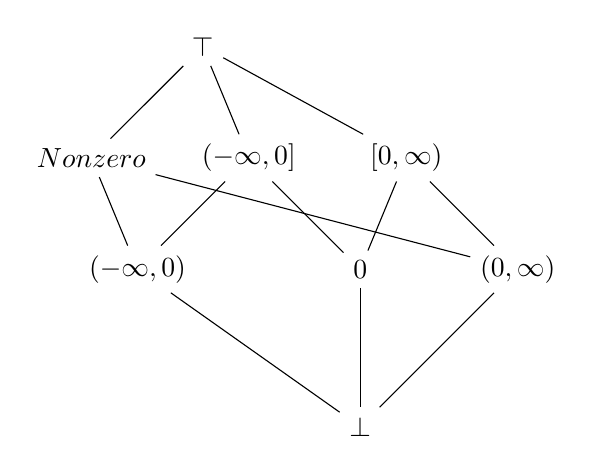
\begin{tikzpicture}[node distance=2cm]
        \node (top) at (0,0) {$\top$};
        \node [below left of=top] (nonzero) {$Nonzero$};
        \node [right of=nonzero] (contains-neg) {$(-\infty, 0]$};
        \node [right of=contains-neg] (contains-pos) {$[0, \infty)$};
        \node [below left of=contains-neg] (neg) {$(-\infty, 0)$};
        \node [below right of=contains-neg] (zero) {$0$};
        \node [below right of=contains-pos] (pos) {$(0,\infty)$};
        \node [below of=zero] (bottom) {$\bot$};
        \draw [black] (top) -- (contains-pos);
        \draw [black] (top) -- (contains-neg);
        \draw [black] (top) -- (nonzero);
        \draw [black] (contains-pos) -- (pos);
        \draw [black] (contains-neg) -- (neg);
        \draw [black] (nonzero) -- (neg);
        \draw [black] (nonzero) -- (pos);
        \draw [black] (contains-pos) -- (zero);
        \draw [black] (contains-neg) -- (zero);
        \draw [black] (pos) -- (bottom);
        \draw [black] (neg) -- (bottom);
        \draw [black] (zero) -- (bottom);
    \end{tikzpicture}
    \caption{Lattice for the signedness analysis}
    \label{fig-signedness}
\end{figure}

\section{Related Work}

There is a large body of work on abstract interpretation and its relationship
with other, similar static analysis techniques, which is far
too extensive to cover here.
For a sample, see Cousot and Cousot~\cite{cousot14}.
The mathematical framework provided by abstract interpretation is sufficiently
general to express most static analyses, including type systems.
As far as we are aware, this work is the first attempt to automatically
create abstract interpretations from a set of examples, but there is a
large body of prior work that makes building static analysis tools easier.
(whether they are based directly on abstract interpretation or not).
The Checker Framework makes building type systems for Java easier
by providing a framework for type system designers~\cite{checker-framework};
because types are an abstract interpretation, the Checker Framework
is a framework for designing and building abstract interpretations.
IKOS is a framework for developing static analyses directly based on
abstract interpretations, developed by NASA for verifying flight
controllers~\cite{ikos}. Modern compilers use a framework for building
the dataflow analyses they use to perform optimizations and code generation
~\cite{lattner04:_llvm}; these dataflow analyses, too, can be viewed as
abstract interpretations. The current state of the art in industry is to
utilize domain specific query languages to describe static analyses, such as 
Semmle's QL, a datalog variant~\cite{semmle-ql-primer}.
These frameworks and others like them make it easier and faster to develop analyses, but 
building a precise, sound analysis still requires an expert.  Our tool 
aims to remove that requirement by automating the development of analyses; 
we could target our tool to generate code that runs in any of these frameworks.

Previous work on abstract interpretation has considered its relationship
with SAT/SMT solvers, which our approach relies on. Brain et al. characterized
DPLL(T), the main algorithm upon which modern SAT/SMT solvers are built,
as an abstract interpretation~\cite{brain2013abstract}. By calling out to
an SMT solver as part of the transfer function, Jiang et al. are able to
improve the refinements made by their abstract
interpretations~\cite{jiang2017block}. The PAGAI static analyzer uses
an SMT solver to more precisely refine path conditions~\cite{pagai}.
While all of these results combine abstract interpretations with
an SAT or SMT solver in some way, none actually use the solver to
synthesize the abstract interpretation.

Counterexample-guided abstraction refinement (CEGAR) is a general technique
for improving verification results~\cite{cegar}. This technique can be
viewed as using a solver to refine an abstract interpretation into a
more precise abstract interpretation, but we are not aware of any
uses of the technique which generate an abstract interpretation from
only user-provided examples. CEGAR has been used in many contexts,
including model checking~\cite{clarke2003counterexample},
test generation~\cite{beyer2004},
and stability analysis~\cite{prabhakar2016counterexample}.

A similar domain is inferring invariants. Verifying a program is straightforward
(and can be mechanized~\cite{hoare69}) if inductive invariants are supplied for
each loop or recursive function, and generating these invariants is
known to be a synthesis problem. Recent work has focused on learning
invariants via a counter-example guided approach~\cite{garg2014ice} or
on guessing invariants via an efficient random search algorithm and then
checking whether they are correct~\cite{sharma2016invariant}.
These approaches still require the programmer to specify the correctness
properties of the system formally; our tool allows developers to specify
the analysis they need with examples. In practice, developers write
test cases like the ones our tool requires, but rarely formally specify
the properties of their systems.

Our approach relies on example-driven synthesis, which has been effectively
applied in other domains. Microsoft's Excel spreadsheet tool can automatically
synthesize programs to transform user input based on a few examples
provided by the user using FlashFill~\cite{flashfill}. Bornholt and
Torlak used litmus tests to synthesize memory models for complex architectures
like x86 and PowerPC~\cite{bornholt17}. Perelman et al. developed a general
framework for synthesizing programs from test cases~\cite{perelman2014test}.
These approaches (and ours) share a general framework: the user provides
some examples of what they are trying to accomplish, and a program
(whether it manipulates a spreadsheet, models the memory architecture of
a processor, or implements an abstract interpretation) is produced
automatically by a solver. Our technique extends approaches like these
to a promising new domain: abstract analyses.

\section{Future Work}
\label{sec-fw}

A conference-length paper on this topic would extend the tool to operate
on Java programs, with the final goal being the replication of
existing Checker Framework checkers using only those checkers'
test suites. This would require building more
complex transfer functions---and probably would require
a meta-sketching approach~\cite{metasketching} which tries several levels of
sketches for the transfer functions (moving from refining only the result of the expression, to
refining multiple variables, to a flow-sensitive refinement, etc.).
This would also require implementing the last stage of the tool, which
translates the synthesized transfer function into a Checker Framework
checker or some other backend. Getting this whole pipeline working would,
we think, be an interesting research contribution, but we are less
confident that the approach is feasible at all, so we intend to start
by validating whether we can produce transfer functions that are
similar to what a human might write before we worry about translating
them into practical analyses.

\section{References}

\begingroup
\renewcommand{\section}[2]{}%

% The following two commands are all you need in the initial runs of
% your .tex file to produce the bibliography for the citations in your
% paper.
\bibliographystyle{plain}
\bibliography{genprog-bib/merged}
% You must have a proper ``.bib'' file
% and remember to run:
% latex bibtex latex latex
% to resolve all references
%
% ACM needs 'a single self-contained file'!
%
\endgroup

\appendix

This appendix contains the test cases used to generate the ``parity0''
analysis discussed in \secref{eval}. The test cases are very simple and
were chosen for convenience.

\begin{lstlisting}
add_evens.imp:
        x = @Both read_int();
        @Even y = 2;
        @Even z = 2 * x;
        return @Even y + z;

add_evens_loop.imp:
        lc = read_int();
        @Even y = 0;
        while (0 < lc){
            @Even y = y + (@Even 2);
            lc = lc -1;
        }
        return y;

if_merge.imp:
        x = @Both read_int();
        y = x;
        if(x < 10) {
            @Odd y = 1;
        } else {
            @Even y = 2;
        }
        return y;

while_merge.imp:
        x = @Both read_int();
        y = x;
        while(0 < x) {
            x = x - @Odd 1;
            @Even y = 2 * y;
        }
        return y;

\end{lstlisting}

\end{document}
This is never printed
